\documentclass[12pt]{article}

% Language setting
\usepackage[utf8]{inputenc}
\usepackage[bulgarian]{babel}

% --------------------- Packages  --------------------
% Use biblatex
\usepackage{biblatex}
\addbibresource{bibliography.bib}
% Table thickness
\usepackage{ctable}
% Equations: SI units
\usepackage{siunitx}
% Approximately equal
\usepackage{amssymb}
% degrees symbol
\usepackage{gensymb}
% warning box
\usepackage{pifont,mdframed}

\newenvironment{warning}
  {\par\begin{mdframed}[linewidth=2pt, linecolor=white]%
    \begin{list}{}{\leftmargin=1cm
                   \labelwidth=\leftmargin}\item[\Large\ding{43}]}
  {\end{list}\end{mdframed}\par}

% --------------------- Title  --------------------
\addbibresource{bibliography.bib}

\begin{document}

% Anfang der Titelseite________________________________________________________________________________
\begin{titlepage}
	\flushleft
% 	\begin{center}
	%{\scshape\Large Werkstoffe III \hspace{2.5cm} Laborbericht \hspace{2.5cm}HS 2022 \par}
	{\scshape\Large Протокол V \hspace{2cm} Механика - практикум\par}
	\vspace{5cm}
	{\huge\bfseries Атвудова машина\par}
	\vspace{1cm}
	{\LARGE\bfseries Лабораторно упражнение №4\par}
	\vspace{5cm}
    % {\LARGE\bfseries Физически Факлутет към Софийски Университет ``Св. Климент Охридски \par}
    {\LARGE\bfseries Виолета Кабаджова, \par}
%   {\LARGE\bfseries Group: X\par}
    {\large\bfseries ККТФ, факл. номер: 3PH0600026\par}
	\vspace{1cm}
	
	{\large Физически Факлутет, 
	
	Софийски Университет "Св. Климент Охридски"
	
	15 ноември 2022 г.\par}
	
\end{titlepage}

\section{Теоритична част}\label{sec:theoretical-part}
Атвудовата машина е уред, чрез който могат да се изследват праволинейни вертикални движения. Схема на такъв уред е показана на фиг. \ref{fig:device} - той представлява макара, от двете страни на която има закачени на нишка две тела с равна маса $m_\tau$. Приемаме, че нишката е неразтеглива и не се хлъзга по макарата. В началото и края на указанато на фигурата разстояние $S_2$ се намира по една фотоклетка, с помощта на които може да се измери времето, за което тялото преминава през горната част на $S_2$ и достига до долната част от уреда, като се удря в основата. На тялото от страната на фотоклетките могат да се поставят пръстени, които нарушават баланса, установен между двете тела в изходното положение, като по този начин създават равноускорително движение.


\begin{figure}
    \centering
    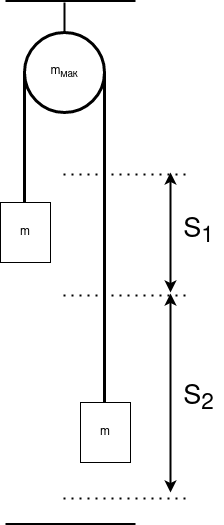
\includegraphics[width=0.2\textwidth]{images/atwood-machine.drawio.png}
    \caption{Атвудова машина}
    \label{fig:device}
\end{figure}

\section{Експериментална част}
\subsection{Експериментална установка}
Освен самото устройство, илюстрирано на фиг. \ref{fig:device}, имаме и общо три пръстена, които могат да се слагат върху тялото, чието време на падане засичаме. Именуваме всеки от пръстените по стандарта П$i$ и записваме съответните пръстени с техните маси в таблица \ref{tbl:rings}. 

\begin{table}[h]
\begin{center}
\begin{tabular}{|l|l|}\hline
име & m_i, [g] \\ \hline
П1 &2.16 \\ \hline
П2 &8.01 \\ \hline
П3 &14.78 \\ \hline
\end{tabular}
\caption{\label{tbl:rings}Пръстените, използвани за допълнителни тежести, и техните маси.}
\end{center}
\end{table}

\subsection{Задача 1: Проверка на закона за пътя при равноускорително движение}
Многократно измерваме времето, за което едното тяло изминава път L=18 cm и L=25 cm. Получените резултати записваме в таблица \ref{tbl:task-1}. Измерванията от 1 до 5 са при $L=S_2=18cm$, а от 6 до 10 - при $L=S_2=25cm$. Законът за пътя при равноускорително движение без начална скорост е $S = \frac{at^2}{2}$. Построявайки графиката на $2S(t^2)$ при дължини на $S_2 = L$ (18 или 25 cm) по Ox и квадрата на средните стойности на измереното време, можем да определим ускорението $a=tan\alpha$, където $\alpha$ е ъгълът, получен при пресичането на графиката с Oх. В горепосочената таблица пресмятаме и ускоренията по закона $S = \frac{at^2}{2}$. Проверяваме този закон като сравняваме стойностите на полученото a от тангенса на ъгъл $\alpha$ и полученото от средните стойности, които трябва да са равни в рамките на грешката.


% \begin{figure}
%     \centering
%     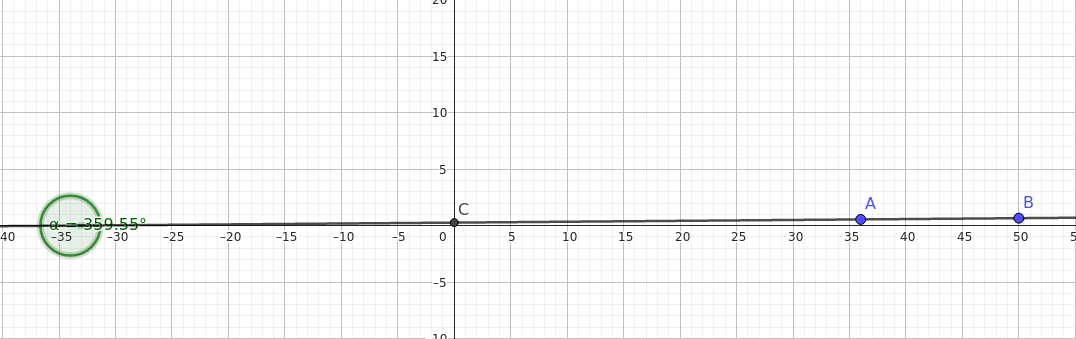
\includegraphics[width=1.2\textwidth]{images/atwood-task-1.png}
%     \caption{Графика на средната стойност на времената (по Ox) за съответната дължина на $S_2 = L$ (по Oy). Тангенсът на ъгъла, получен при пресичането на графиката с Oх трябва да ни даде пресметнатото средно ускорение за съответната дължина}
%     \label{fig:task1-graph}
% \end{figure}

\begin{table}[h]
\begin{center}
\begin{tabular}{|l|l|l|}\hline
N & t_i, [s] &a_i, [m/s] \\ \hline
\specialrule{.1em}{0em}{.2em}
1 &0.589 &1.038 \\ \hline
2 &0.518 &1.342 \\ \hline
3 &0.556 &1.165 \\ \hline
4 &0.570 &1.108 \\ \hline
5 &0.524 &1.311 \\ \hline
\specialrule{.1em}{0em}{0em}
6 &0.656 &1.162 \\ \hline
7 &0.693 &1.041 \\ \hline
8 &0.648 &1.191 \\ \hline
9 &0.641 &1.217 \\ \hline
10 &0.658 &1.155 \\ \hline
\specialrule{.1em}{0em}{0em}
& \bar{t}_{1-5} = 0.551 s & \bar{a}_{1-5} = 1.193 s \\ \hline
& \bar{t}_{6-10} = 0.659 s & \bar{a}_{6-10} = 1.153 s \\ \hline
\end{tabular}
\caption{Направени измервания на височини L=18cm и L=25cm.}
\label{tbl:task-1}
\end{center}
\end{table}


За средна стойност на ускорението от получените стойности в таблицата получаваме $a = 1.173 \frac{m}{s^2}$. Също така знаем, че:

\begin{equation}\label{eq:theoretical-task1}
    g = \frac{2m_T + m_\Pi}{m_\Pi} a   
\end{equation}

От уравнение \ref{eq:theoretical-task1} получаваме, че теоритичната стойност за а e $0.87 \pm 0.14 \frac{m}{s^2}$, равно на получената от експерименталните данни стойност $1.17 \pm 0.16 \frac{m}{s^2}$ в рамките на грешките им, откъдето и доказваме закона за равноускорително движение.


\subsection{Задача 2: Измерване на стойността на земното ускорение}
Фиксираме $S_2 = 20 cm$, $S_1 = 15 cm$. От пръстените, описани в таблица \ref{tbl:rings}, избираме следните три комбинации от пръстени: П3, П2, П1+П2. Записваме измерванията в таблици \ref{tab:ring3-meas}, \ref{tab:ring2-meas} и \ref{tab:ring12-meas}.

Докато тялото пада надолу с допълнителните си тежести, то се движи равноускорително без начална скорост (от състояние на покой), което означава, че тялото се движи равноускорително в сектор $S_1 = \frac{at^2}{2}$. При достигане на началната точка от пътя $S_2$ обаче (виж фиг. \ref{fig:device}) тялото започва да се движи равномерно по закона $S_2 = vt$.

От закона за пътя при равномерно праволинейно движение се получава $S_1 = \frac{at_1^2}{2}, v_1 = at_1, S_2 = v_1t_2$, където $t_1$, $t_2$ са времената за изминаване на съответните разстояния $S_1$ и $S_2$. От тези уравнения изключваме $t_1$ за равноускорителното движение, което не можем да измерим поради липсата на фотоклетки и изразяваме $a$ само чрез $S_1, S_2, t_2$ (формула \ref{eq:a-task2}), откъдето следва и формула \ref{eq:g-task2}. Следователно формулата за абсолютна грешка за земното ускорение ще бъде посочената в уравнение \ref{eq:g-error}.

\begin{equation}\label{eq:a-task2}
    a = \frac{S_2^2}{2S_1t_2^2}
\end{equation}

\begin{equation}\label{eq:g-task2}
g = \frac{(2m_\tau + m_j)S_2^2}{2m_jS_1t_2^2}    
\end{equation}

\begin{equation}\label{eq:g-error}
    \Delta g = \pm g(\frac{2\Delta m_T + \Delta m_j}{2m_T + m_j} + 2\frac{\Delta S_2}{S_2} + \frac{S_1}{S_1} + \frac{\Delta m_j}{m_j} + 2\frac{\Delta t_2}{t_2})
\end{equation}

\begin{table}
    \centering
    \begin{tabular}{|l|l|l|} \hline
    N &t_i, [s] &(t_i-\bar{t}_{\Pi3})^2\cdot10^{-3} \\ \hline
    1 &0.38 &0.001 \\ \hline
    2 &0.383 &0.016 \\ \hline
    3 &0.381 &0.004 \\ \hline
    4 &0.377 &0.004 \\ \hline
    5 &0.376 &0.009 \\ \hline
    \specialrule{.1em}{0em}{0em}
    & \bar{t}_{\Pi3} = 0.379 & g_{\Pi3} = 8.425 \pm 2.861\\ \hline
    \end{tabular}
    \caption{Измервания за експеримент с добавена тежест П3, чиято маса се причислява на 14.78 g.}
    \label{tab:ring3-meas}
\end{table}

\begin{table}
    \centering
    \begin{tabular}{|l|l|l|} \hline
    N &t_i, [s] &(t_i-\bar{t}_{\Pi2})^2\cdot10^{-3} \\ \hline
    6 &0.499 &0.009 \\ \hline
    7 &0.489 &0.049 \\ \hline
    8 &0.498 &0.004 \\ \hline
    9 &0.494 &0.004 \\ \hline
    10 &0.502 &0.036 \\ \hline
    \specialrule{.1em}{0em}{0em}
    & \bar{t}_{\Pi2} = 0.496 & g_{\Pi2} = 8.528 \pm 2.923\\ \hline
    \end{tabular}
    \caption{Измервания за експеримент с добавена тежест П2, чиято маса се причислява на 8.01 g.}
    \label{tab:ring2-meas}
\end{table}

\begin{table}
    \centering
    \begin{tabular}{|l|l|l|} \hline
    N &t_i, [s] &(t_i-\bar{t}_{\Pi12})^2\cdot10^{-3} \\ \hline
    11 &0.448 &0.036 \\ \hline
    12 &0.444 &0.1 \\ \hline
    13 &0.456 &0.004 \\ \hline
    14 &0.458 &0.016 \\ \hline
    15 &0.464 &0.1 \\ \hline
    \specialrule{.1em}{0em}{0em}
    & \bar{t}_{\Pi12} = 0.454 & g_{\Pi12} = 8.239 \pm 2.896\\ \hline
    \end{tabular}
    \caption{Измервания за експеримент с добавена тежест П2 + П1, чиято обща маса става 10.17 g.}
    \label{tab:ring12-meas}
\end{table}

От таблиците с измервания \ref{tab:ring3-meas}, \ref{tab:ring2-meas} и \ref{tab:ring12-meas} пресмятаме средните времена за преминаване през $S_2$. Откъдето получаваме и стойностите за земното ускорение g по формула \ref{eq:g-task2} със съответните грешки по формула \ref{eq:g-error}.

Получените стойности за g можем да поставим на графика, по Ox оста, на която ще разположим $\frac{1}{m}$, а по Oy - съответното получено g. Прекарвайки медиана между тези точки, екстраполираме и получаваме стойността на g в пресечната точка с Оу (това действие е показано на фиг. \ref{fig:extrapolation-graph}). Графиката пресича Oy в $g = 8.24 \frac{m}{s^2}$. Причината да получаваме g, толкова по-малко от очакваното е, че Нютоновата механика е създадена за тела с големи маси, докато тези в текущата лаборатория са ограничени до 1 kg, което на практика води до това много от силите, които пренебрегваме (като триене между макарата и нишката), в същност да се оказват съществетни.


\begin{figure}
    \centering
    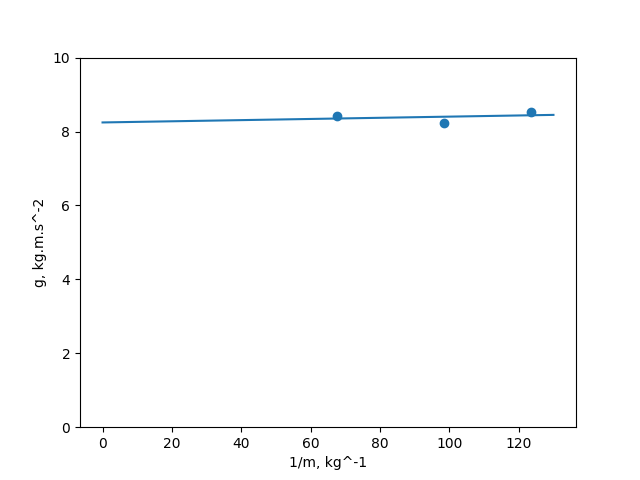
\includegraphics[width=0.6\textwidth]{images/task2.png}
    \caption{Графика на екстраполацията, пресичаща 0y в точка с координати (0, 8.24) }
    \label{fig:extrapolation-graph}
\end{figure}



\end{document}
